\documentclass[lettersize,journal]{IEEEtran}
\usepackage{amsmath,amsfonts}
\usepackage{algorithmic}
\usepackage{array}
\usepackage[caption=false,font=normalsize,labelfont=sf,textfont=sf]{subfig}
\usepackage{textcomp}
\usepackage{stfloats}
\usepackage{url}
\usepackage{hyperref}
\usepackage{verbatim}
\usepackage{graphicx}
\usepackage{tikz}
\usetikzlibrary{shapes,arrows,positioning}
\hyphenation{op-tical net-works semi-conduc-tor IEEE-Xplore}
\def\BibTeX{{\rm B\kern-.05em{\sc i\kern-.025em b}\kern-.08em
    T\kern-.1667em\lower.7ex\hbox{E}\kern-.125emX}}
\usepackage{balance}
\begin{document}
\title{Comparative Empirical Evaluation of Software Test Automation using Artificial Intelligence and Manual Test Case Design}
\author{Jesús José Bone Caicedo, José Luis Carvajal Carvajal, and Victor Xavier Quiñonez Ku
\thanks{J. J. Bone Caicedo, J. L. Carvajal Carvajal, and V. X. Quiñonez Ku are with the Systems and Software Department, Pontifical Catholic University of Ecuador Esmeraldas Campus, Esmeraldas Ecuador (e-mail: jjbone@pucese.edu.ec; jose.carvajal@pucese.edu.ec; xavier.quinonez@pucese.edu.ec).}}

\markboth{Journal of Software Engineering Research,~Vol.~1, No.~1, 2025}%
{Bone Caicedo et al.: Comparative Empirical Evaluation of Software Test Automation}

\maketitle

\begin{abstract}
This study presents an empirical comparison between manually designed test cases and those automatically generated by generative artificial intelligence tools---ChatGPT and Diffblue Cover---applied to the Spring PetClinic system, developed in Java and Spring Boot. The fully automated experiment comprised 2,480 runs distributed across 12 test classes (6 human and 6 AI-generated), with 40 iterations per class and a total duration of 6.18 hours. Four main metrics---instruction coverage, branch coverage, mutation score, and execution time---were evaluated using descriptive and inferential analysis (Student's t, Welch, and Mann-Whitney U). At the aggregate level (N = 12), no significant differences were found ($p > 0.05$; $d < 0.30$), while at the complete level (N = 2,480), small effects ($r < 0.15$) were observed in all metrics, indicating marginal differences between the two approaches. The results confirm that generative AI can achieve quantitative performance comparable to that of human testing, albeit with more limited functional reasoning. This work provides empirical evidence on the current capabilities and limitations of AI in automated testing, highlighting its potential to accelerate repetitive tasks and improve productivity without replacing human analytical judgment.
\end{abstract}

\begin{IEEEkeywords}
automated testing, Diffblue Cover, generative AI, software quality, test case generation
\end{IEEEkeywords}


\section{Introduction}
\IEEEPARstart{I}{n} the context of digital transformation and the growing incorporation of artificial intelligence in all stages of the software life cycle, test automation has taken center stage in agile development processes due to its potential to increase coverage, reduce time, and improve product reliability. This technical advance not only responds to a need for efficiency in engineering teams, but also to social demand for more reliable, secure, and highly available digital services, whose quality has a direct impact on sensitive sectors such as health, education, and finance. The emergence of generative AI---with large language models (LLMs) and associated tools---has renewed this field by promising faster and assisted test case generation, albeit with mixed and context-dependent results \cite{Trudova2020, Garousi2025, Singh2023, Li2025}. In ecosystems dominated by Java and Spring Boot, it is pertinent to subject these solutions to rigorous evaluation to establish their true scope and limitations compared to traditional approaches \cite{Trudova2020, Garousi2025}.

Despite recent advances (e.g., improvements in LLM-assisted unit testing in industrial contexts) \cite{Alshahwan2024}, the literature shows that the landscape is still fragmented. Research such as that by Schäfer et al. \cite{Schfer2023} and Yang et al. \cite{Yang2024} has demonstrated the ability of LLMs to generate automatic unit tests with promising results, but without establishing direct comparisons with human tests. Complementarily, Bhatia et al. \cite{Bhatia2024} empirically evaluated the performance of ChatGPT against traditional tools such as Pynguin, showing comparable or superior coverage, but also a significant proportion of incorrect assertions and dependence on human supervision. Similarly, Kanth et al. \cite{RoshniKanth2023} contrast conventional methodologies and AI-based approaches, focusing their analysis on efficiency and coverage, although without strict control over a common system under test (SUT). For their part, Kirinuki and Tanno \cite{Kirinuki2024} evaluated the interaction between ChatGPT and human testers in black-box testing, highlighting qualitative differences in reasoning and understanding of the system. However, recent systematic and grey literature reviews, such as that by Ricca et al. \cite{Ricca2025}, agree that there is still a lack of empirical evidence combining standardized quantitative metrics---such as mutation score or coverage---with functional observations in the same experimental environment. While recent works have explored advanced metric-driven approaches, such as mutation-guided test generation \cite{Wang2025}, these efforts remain largely focused on quantitative effectiveness rather than functional interpretation.

In this context, an empirical gap persists: there is a lack of systematic and quantitative comparisons between AI-generated tests and manually designed tests under the same SUT and replicable evaluation framework \cite{Garousi2025}. Although the literature reports benefits---faster generation and automated exploration---it also warns of limitations associated with variable quality, false positives, and dependence on human supervision \cite{Junior2023, Rehan2025, Huang2025}. This combination of advances and gaps justifies the need for controlled studies that contrast the actual effectiveness of both approaches under equivalent conditions.

In addition to traditional quantitative indicators, this study incorporates a complementary observation related to functional understanding, understood in empirical terms as the differences observed in the way the compared approaches---generative AI and manual design---address the logic and functionality of the system under test. This dimension does not seek a formal cognitive analysis, but rather to contextualize the numerical results (coverage, mutation score, efficiency) based on how each approach interprets and structures the test cases \cite{Garousi2025, Li2025, Rehan2025, Huang2025}. Its inclusion enriches the reading of the findings, offering a more complete perspective on the performance and functional quality of the automated testing process.

This study aims to evaluate, in a controlled environment, the effectiveness of test cases automatically generated by generative AI compared to those manually created in Java projects, using a representative Java/Spring Boot project as the system under test (SUT). The overall objective of the study is to evaluate the effectiveness and functional understanding, from an empirical approach, of AI-generated test cases compared to those designed by humans, combining quantitative metrics---coverage (instruction/branch), mutation score, and operational efficiency---with empirical observations on their ability to adequately represent the functionality of the system \cite{Gkikopouli2023}.

The expected contribution integrates comparative evidence with replicable metrics and an analytical component that considers the empirical perspective of functional understanding, offering useful inputs for decision-making in educational and professional settings \cite{Trudova2020, Alshahwan2024}. In line with this technical and social relevance, the research adopts a comparative experimental approach, based on objective metrics and empirical observations, which allow for the examination of both the quantitative performance and the interpretive quality of AI-generated tests compared to manual tests in a controlled environment. Finally, the article is structured as follows: section 2 describes the materials and methods; section 3 presents the results and discussion; and section 4 develops the conclusions and future projections.   



\section{Materials and Methods}

\subsection{Research Design}

The study was developed under a mixed-method empirical-comparative design, aimed at evaluating the effectiveness and functional understanding of test cases generated by generative artificial intelligence versus those developed manually. An applied approach was adopted, focused on measuring the actual performance of automatic verification techniques in a software quality assurance context. The experiment was conducted between May and December 2025 in a controlled academic environment, using the open-source Spring PetClinic project as the system under test (SUT) due to its modular structure, stability, and widespread use in empirical research \cite{Garousi2025}. Two test suites were generated from this SUT: one using generative AI tools (ChatGPT Plus and Diffblue Cover CLI) and another manually created by the researcher. Both were evaluated under equivalent conditions using standardized quantitative metrics (code coverage, mutation score, and execution time) and a qualitative analysis aimed at understanding the functional aspects of the system.

The methodological design followed contemporary guidelines for empirical studies with language models, which recommend documenting versions, configurations, prompts, and interactions to ensure transparency, reproducibility, and traceability \cite{Baltes2025}. Recent guidelines on the role of LLMs in software engineering research were also incorporated, emphasizing the importance of maintaining human oversight, explicitly declaring the use of AI-based tools, and mitigating the methodological risks associated with their use \cite{Trinkenreich2025}. These principles made it possible to control external variables, strengthen the internal validity of the study, and ensure that the results were verifiable and replicable through the use of professional tools in controlled and documented versions.

\subsection{Materials and Experimental Environment}

The study was conducted entirely on the Spring PetClinic system (Java 17, Spring Boot 3.5.6, 3.5.0-SNAPSHOT), selected as the sole system under test (SUT) due to its adoption in recent research, its modular architecture, and its compatibility with automation frameworks in Java \cite{Garousi2025}. Since the research did not involve human subjects, the researcher's intervention was limited to the design and technical execution of manual tests, while the artifacts analyzed corresponded exclusively to test cases generated by artificial intelligence and manually designed tests under controlled conditions. The manual tests were developed using functional exploration with Postman and coded in JUnit 5 and MockMvc, while the AI-generated cases were obtained using ChatGPT (GPT-5 model) and Diffblue Cover CLI (Teams Edition), the latter executed without human intervention to ensure neutrality in bytecode-based generation. Additionally, automation scripts in PowerShell were used to sequentially and reproducibly execute the functional, unit, and combined test suites, avoiding manual intervention during execution.

Quantitative metrics were collected using JaCoCo 0.8.12 (instruction and branch coverage), PITest 1.16.0 (mutation score), and Maven Surefire 3.2.5 (total execution time), with automatic export of results in XML, CSV, and HTML formats. Python 3.12.6 was used for statistical analysis with the pandas, numpy, scipy, matplotlib, seaborn, and openpyxl libraries, allowing the calculation of descriptive measures, normality and variance contrasts, hypothesis tests (Shapiro-Wilk, Levene, Student's t-test, Mann-Whitney U) and effect sizes (Cohen's d and r). All runs were performed on a computer with an Intel Core i7-12700KF processor, 32 GB DDR4 RAM, and 1 TB NVMe SSD, running Windows 11 Pro 23H2, without parallel loads and with fixed random seeds to ensure determinism and reproducibility, in accordance with recent guidelines for AI-assisted empirical studies in software engineering \cite{Ricca2025, Baltes2025}.

The experimental sample consisted of test suites produced using both approaches: functional and unit tests generated by AI (ChatGPT and Diffblue Cover) and equivalent tests designed manually on the same SUT components. This configuration allowed for an objective comparison of coverage, mutation, and operational efficiency metrics, complemented by qualitative observations on the functional consistency of the cases. All configurations, parameters, versions, and resulting artifacts were documented in a supplementary technical record to facilitate future replication of the experiment.

\subsection{Experimental Protocol}

The experimental protocol was developed in five consecutive phases, with the aim of ensuring methodological consistency, variable control, and reproducibility. In the planning phase, an initial literature review was conducted on artificial intelligence-assisted test automation techniques, and the study's comparison criteria were defined based on the selected metrics: instruction coverage, branch coverage, mutation score, and execution time. At the same time, the system under test (Spring PetClinic) was selected as the base environment for the empirical evaluation of manual and AI-generated approaches.

During the preparation phase of the experimental environment, the SUT was configured and the necessary measurement instruments for collecting metrics (PITest and Surefire) were installed, while JaCoCo was already part of the original project configuration. Subsequently, test cases were generated for the three approaches analyzed: (i) tests generated by ChatGPT GPT-5 using neutral prompts and providing only the source code of the method; (ii) unit tests automatically generated by Diffblue Cover CLI, without human intervention; and (iii) manual tests designed by the researcher with JUnit 5 and MockMvc, derived from the inspection of the source code and the behavior observed during the previous functional exploration with Postman.

The automated execution phase of the experiment was implemented using three PowerShell scripts, whose internal names were kept unchanged, supplemented with a brief description for clarity. The run\_pitest\_isolated\_complete.ps1 script (responsible for executing all unit tests for both approaches) performed 40 consecutive iterations, recording the metrics from JaCoCo, PITest, and Surefire in each one. Similarly, the run-test-metrics.ps1 script (responsible for functional testing) ran 40 additional iterations under the same measurement conditions. Finally, the run\_all\_metrics\_simple.ps1 script acted as an orchestrator, coordinating the sequential execution of the two previous scripts and recording the overall time of the process. In all cases, three preliminary runs (warm-up runs) were included to stabilize the JVM and mitigate the variability associated with the initial startup.

During the recording and organization of results phase, the outputs generated by each iteration---including XML files, CSV files, and HTML reports---were structured into separate directories by test type (functional or unit) and by approach (AI or manual), maintaining consistent names and fixed paths to ensure traceability. No human intervention was allowed during automated execution, and execution parameters, seeds, paths, and configurations were kept constant in order to minimize experimental noise and reinforce the internal validity of the study.

In the final phase of statistical analysis, the collected data were processed in Python using the pandas, numpy, scipy, seaborn, and matplotlib libraries. Descriptive measures (mean, median, standard deviation) were calculated, and statistical assumptions were verified using the Shapiro-Wilk (normality) and Levene (homogeneity of variances) tests. Depending on the fulfillment of these assumptions, parametric (Student's t-test or Welch's correction) or nonparametric (Mann-Whitney U) significance tests were applied. Effect sizes (Cohen's d and r) were also calculated, and graphical representations were generated to support the results obtained and facilitate their comparative interpretation. 

The complete flow of the experimental protocol is presented in Fig.~\ref{fig:experimental-protocol}.

\begin{figure}[htb]
\centering
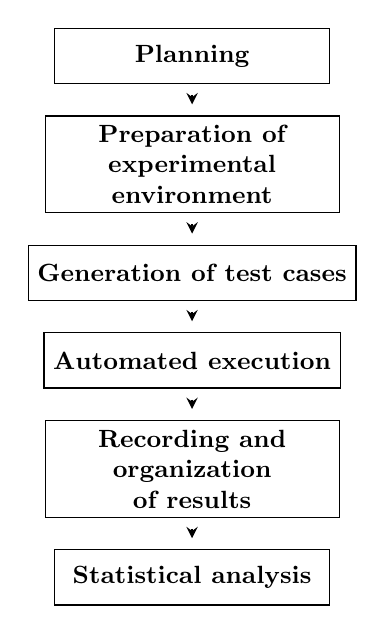
\begin{tikzpicture}[
  node distance=0.4cm,
  auto,
  box/.style={
    rectangle,
    draw=black,
    fill=white,
    text=black,
    minimum width=3.5cm,
    minimum height=0.7cm,
    font=\small\bfseries,
    text centered
  },
  arrow/.style={
    ->,
    thick,
    draw=black,
    shorten <=4pt,
    shorten >=4pt,
    >=stealth
  }
]

\node[box] (planning) {Planning};
\node[box, below=of planning] (prep) {\parbox{3.5cm}{\centering Preparation of experimental \\ environment}};
\node[box, below=of prep] (generation) {Generation of test cases};
\node[box, below=of generation] (execution) {Automated execution};
\node[box, below=of execution] (recording) {\parbox{3.5cm}{\centering Recording and organization \\ of results}};
\node[box, below=of recording] (analysis) {Statistical analysis};

\draw[arrow] (planning) -- (prep);
\draw[arrow] (prep) -- (generation);
\draw[arrow] (generation) -- (execution);
\draw[arrow] (execution) -- (recording);
\draw[arrow] (recording) -- (analysis);

\end{tikzpicture}
\caption{\label{fig:experimental-protocol}Workflow representing the experimental protocol followed during the study.}
\end{figure}
\vspace{-0.5em}

\subsection{Variables and Metrics}

The study defined a set of independent and dependent variables aimed at comparing the behavior of test cases generated using artificial intelligence with those designed manually. The independent variable (IV) corresponded to the test generation approach, established with two levels: (i) manual generation and (ii) generation assisted by generative AI. The dependent variables (DV) were the results obtained from the quantitative and qualitative metrics used to evaluate the performance of both approaches, according to criteria identified in recent evaluations of AI-assisted testing tools \cite{Garousi2025, Ricca2025}.

Among the quantitative variables, three main metrics were considered. Code coverage was evaluated using the indicators instruction coverage and branch coverage, in order to measure the percentage of instructions and paths executed by each test suite. The robustness of the test suite was measured using the mutation score, a widely used indicator for estimating the ability of tests to identify intentional modifications in the source code \cite{Garousi2025}. Finally, operational efficiency was defined as the total execution time of each test suite under controlled conditions, allowing for a comparison of the time load associated with each approach.

In addition to these quantitative metrics, a qualitative variable called functional comprehension was incorporated, related to the degree of consistency with which each approach represents the internal logic of the system under test. This dimension made it possible to contrast the structural and semantic adequacy of the test cases generated, taking into account recent findings on inconsistencies, omissions, or functional deviations observed in tests generated using language models \cite{Kirinuki2024, Junior2023}. The conceptual structure linking the independent variable with the dependent variables, both quantitative and qualitative, is summarized in Fig.~\ref{fig:variables-metrics}.

\begin{figure}[htb]
\centering
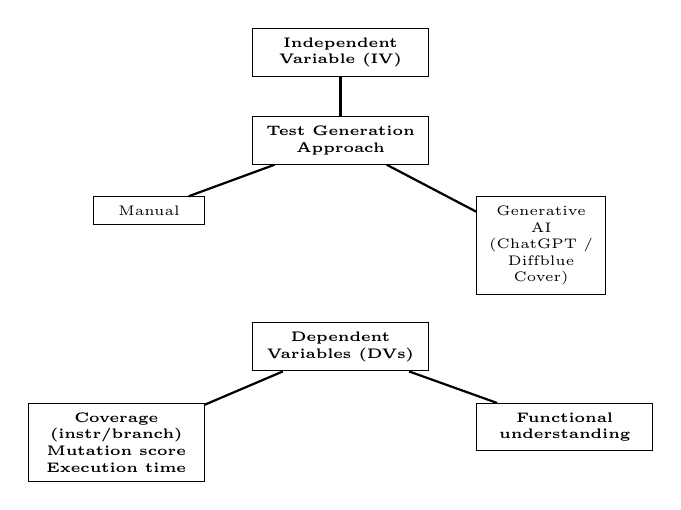
\begin{tikzpicture}[
  node distance=0.5cm,
  auto,
  scale=0.75,
  scale=0.85,
  box/.style={
    rectangle,
    draw=black,
    fill=white,
    text=black,
    minimum width=2.0cm,
    minimum height=0.45cm,
    font=\tiny\bfseries,
    text centered
  },
  smallbox/.style={
    rectangle,
    draw=black,
    fill=white,
    text=black,
    minimum width=1.4cm,
    minimum height=0.35cm,
    font=\tiny,
    text centered
  },
  arrow/.style={
    ->,
    thick,
    draw=black,
    shorten <=3pt,
    shorten >=3pt,
    >=stealth
  }
]

% Independent Variable
\node[box] (iv) {\parbox{2.0cm}{\centering Independent \\ Variable (IV)}};

% Test Generation Approach
\node[box, below=of iv] (tga) {\parbox{2.0cm}{\centering Test Generation \\ Approach}};

% Manual and AI levels
\node[smallbox, below left=0.4cm and 0.6cm of tga] (manual) {Manual};
\node[smallbox, below right=0.4cm and 0.6cm of tga] (ai) {\parbox{1.4cm}{\centering Generative AI \\ (ChatGPT / \\ Diffblue Cover)}};

% Dependent Variables
\node[box, below=2.0cm of tga] (dv) {\parbox{2.0cm}{\centering Dependent \\ Variables (DVs)}};

% Quantitative and Qualitative sections
\node[box, below left=0.4cm and 0.6cm of dv] (quant) {\parbox{2.0cm}{\centering Coverage (instr/branch) \\ Mutation score \\ Execution time}};
\node[box, below right=0.4cm and 0.6cm of dv] (qual) {\parbox{2.0cm}{\centering Functional \\ understanding}};

% Lines from IV
\draw[thick,draw=black] (iv) -- (tga);
\draw[thick,draw=black] (tga) -- (manual);
\draw[thick,draw=black] (tga) -- (ai);

% Lines to DV
\draw[thick,draw=black] (dv) -- (quant);
\draw[thick,draw=black] (dv) -- (qual);

\end{tikzpicture}
\caption{\label{fig:variables-metrics}Conceptual diagram showing the relationships between the independent variable (test generation approach) and the dependent variables (quantitative and qualitative metrics).}
\end{figure}
\vspace{-0.5em}

\subsection{Data Analysis Methods}

The data was analyzed using a quantitative and inferential approach, aimed at comparing the behavior of test cases generated by artificial intelligence with those designed manually. The metrics obtained—instruction coverage, branch coverage, mutation score, and execution time—were processed and organized into comparative tables, accompanied by statistical visualizations such as bar charts, box plots, and violin plots. These analyses were developed using Python and the pandas, numpy, matplotlib, and seaborn libraries.

First, descriptive statistics were applied to calculate measures of central tendency (mean and median) and dispersion (standard deviation) for each metric evaluated. Subsequently, an inferential analysis was performed to identify statistically significant differences between the test generation approaches. To this end, the assumption of normality was verified using the Shapiro-Wilk test and the homogeneity of variances using the Levene test.

The selection of statistical tests depended on the fulfillment of these assumptions. When the metrics met normality and presented homogeneous variances, the classic Student's t-test for independent samples was applied. In cases where normality existed but variances were not homogeneous, Welch's t-test was used. When the metrics did not meet the normality assumption in any of the groups, the nonparametric Mann-Whitney U test was used. In all cases, a significance value of $p < 0.05$ was adopted, accompanied by 95\% confidence intervals.

Finally, effect sizes were calculated to complement the statistical interpretation. Cohen's d was used in comparisons made with Student's t-test, and the r measure was used for comparisons based on the Mann-Whitney U test. The combination of descriptive statistics, parametric and nonparametric tests, and effect size calculations ensured a robust, reproducible analysis consistent with best methodological practices in empirical software engineering studies \cite{Garousi2025, Ricca2025, Huang2025}. The decision flowchart used to select the appropriate statistical test is shown in Fig.~\ref{fig:data-analysis}.

\begin{figure}[htb]
\centering
\resizebox{\columnwidth}{!}{%
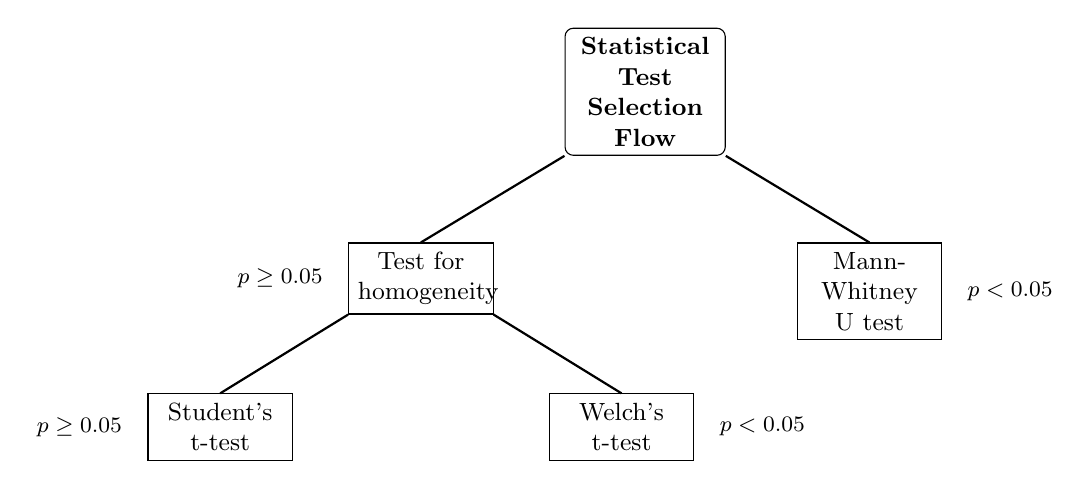
\begin{tikzpicture}[
  node distance=0.6cm,
  auto,
  box/.style={
    rectangle,
    draw=black,
    fill=white,
    text=black,
    minimum width=1.8cm,
    minimum height=0.45cm,
    font=\small\bfseries,
    text centered,
    rounded corners=3pt
  },
  databox/.style={
    rectangle,
    draw=black,
    fill=white,
    text=black,
    minimum width=1.6cm,
    minimum height=0.4cm,
    font=\small,
    text centered
  },
  line/.style={
    thick,
    draw=black
  }
]

% Start node
\node[box] (start) {\parbox{1.8cm}{\centering Statistical Test \\ Selection Flow}};

% Left branch: p >= 0.05
\node[databox, below left=1.1cm and 0.9cm of start] (homogeneity) {\parbox{1.6cm}{\centering Test for \\ homogeneity}};
\draw[line] (start.south west) -- (homogeneity.north);
\node[left=0.2cm of homogeneity, anchor=east] {\footnotesize $p \geq 0.05$};

% Right branch: p < 0.05
\node[databox, below right=1.1cm and 0.9cm of start] (mw) {\parbox{1.6cm}{\centering Mann-Whitney \\ U test}};
\draw[line] (start.south east) -- (mw.north);
\node[right=0.2cm of mw, anchor=west] {\footnotesize $p < 0.05$};

% Bottom left: p >= 0.05
\node[databox, below left=1.0cm and 0.7cm of homogeneity] (student) {\parbox{1.6cm}{\centering Student's \\ t-test}};
\draw[line] (homogeneity.south west) -- (student.north);
\node[left=0.2cm of student, anchor=east] {\footnotesize $p \geq 0.05$};

% Bottom right: p < 0.05
\node[databox, below right=1.0cm and 0.7cm of homogeneity] (welch) {\parbox{1.6cm}{\centering Welch's \\ t-test}};
\draw[line] (homogeneity.south east) -- (welch.north);
\node[right=0.2cm of welch, anchor=west] {\footnotesize $p < 0.05$};

\end{tikzpicture}%
}
\caption{\label{fig:data-analysis}Decision flowchart for selecting the appropriate statistical test based on normality and variance homogeneity assumptions.}
\end{figure}

\subsection{Validity and Reliability Control}

Internal validity was ensured by conducting the experiment in a controlled environment, keeping hardware, software, and system configuration conditions constant. The measurement tools—JaCoCo, PITest, and Surefire—operated autonomously with respect to the origin of the test cases, which made it possible to avoid instrumental biases and ensure a partially blind evaluation. The source code of the system under test was not modified, and the original tests of the project were excluded, preserving the experimental integrity. To reinforce construct validity, widely accepted metrics in software engineering—instruction coverage, branch coverage, and mutation score—were used, identified as consistent indicators for evaluating the quality and effectiveness of AI-assisted testing in recent studies \cite{Garousi2025, Ricca2025, Huang2025}, and consistent with contemporary methodological guidelines for empirical research with generative models \cite{Baltes2025}.

In terms of reliability, controls were implemented to minimize researcher influence. The prompts used in ChatGPT were formulated in a neutral manner, without examples or guidelines, and the tests generated by Diffblue Cover and those designed manually were developed completely independently, avoiding code transfers or adaptations between approaches. Errors or failures observed during execution were recorded without subsequent corrections, ensuring traceability and consistency. External validity was supported by the use of Spring PetClinic, a representative and widely adopted system in empirical evaluations of testing tools for Java/Spring Boot environments, facilitating replication of the study and reinforcing the comparability of the results obtained.

\subsection{Reproducibility and Ethics}

The research was conducted under principles of transparency and traceability, ensuring that the experiment could be replicated in its entirety. All scripts, configurations, execution parameters, and intermediate results were documented and stored in a repository derived from the Spring PetClinic project, maintained under version control and structured to allow complete reproduction of the experimental flow. The system under test was used in accordance with its open source license (Apache 2.0) and without modifications to its source code, ensuring the consistency of the environment and the stability of the evaluation conditions. Likewise, the tools used—including ChatGPT and Diffblue Cover—were executed in accordance with their respective terms of use, avoiding any manipulation or intentional bias in the results.

From an ethical perspective, the study did not involve human participants or the processing of personal data, and therefore did not require informed consent procedures or review by an ethics committee. However, a strict commitment to academic integrity, transparent communication of findings, and the absence of selective exclusion of data was maintained. Generative artificial intelligence was used with neutral prompts and without interventions intended to influence the results, so that the test sets produced reflected the genuine behavior of each tool.

To ensure complete reproducibility of the study, the repository used during the experiment—containing all scripts, configurations, and results—is publicly available at: \href{https://github.com/solveighty/spring-petclinic-test/}{https://github.com/solveighty/spring-petclinic-test/}

\section{Results}

\subsection{Experiment Execution and Dataset Structure}

The experimental execution was carried out using a fully automated process, designed to ensure consistency and eliminate any human intervention during data collection. Forty iterations were performed for each of the 12 test classes considered in the study—six designed manually and six generated using artificial intelligence tools (ChatGPT and Diffblue Cover)—yielding a total of 480 base measurement cycles. The entire execution process took 6.18 hours, considering the valid iterations and preliminary executions used to stabilize the JVM. Each cycle generated two separate records, corresponding to the compilation and execution phases, resulting in a final set of 2,480 raw records. For each record, four metrics were automatically stored: instruction coverage, branch coverage, mutation score, and execution time, extracted directly from the XML, CSV, and HTML artifacts generated by JaCoCo, PITest, and Surefire. Table~\ref{tab:dataset-overview} provides a summary of the experimental dataset structure.

\begin{table}[!h]
\caption{\label{tab:dataset-overview}Summary of the experimental dataset collected during the study.}
\centering
\footnotesize
\begin{tabular}{| p{2.5cm} | p{1.0cm} | p{2.8cm} |}
\hline
Component & Cant. & Details \\
\hline
Total test classes & 12 & 6 Manual + 6 AI-Generated \\
\hline
Iterations per class & 40 & Includes warm-up (3 initial iterations) \\
\hline
Total raw records & 2,480 & 1,600 manuals and 880 AI \\
\hline
Metrics per record & 4 & instruction\%, branch\%, mutation\%, time(s) \\
\hline
\end{tabular}
\end{table}

During the dataset integrity check, it was confirmed that the 2,480 expected measurements were generated correctly, with no missing records, duplicates, or format inconsistencies. The identification labels for each approach (manual and AI) remained consistent across all iterations, and the exported files retained the expected structure for statistical processing. Mutation score values equal to 0 were observed in some cases; however, these correspond to valid runs in which the test sets failed to kill any mutations generated by PITest. All values were retained in their entirety due to their analytical relevance, ensuring the completeness, consistency, and reliability of the dataset used in the following stages of the study.

\subsection{Preparing the Dataset}

The raw records generated during the experimental run—originally stored in twelve CSV files corresponding to the manual and AI-generated test classes—were consolidated into a single master file, following the procedure described in the experimental protocol. This integration was performed using automated Python scripts (pandas), which included format normalization, column name standardization, and data type verification, fully preserving the metrics collected in each iteration and ensuring the structural consistency of the dataset.

For the subsequent stages of the analysis, two levels of aggregation were defined. Table~\ref{tab:data-manuals-ia-overview} illustrates the structure and distribution of records at both aggregation levels.

\begin{table}[!h]
\caption{\label{tab:data-manuals-ia-overview}Total records for each test team.}
\centering
\footnotesize
\begin{tabular}{| p{2.0cm} | p{0.9cm} | p{0.4cm} | p{2.5cm} |}
\hline
Analysis level & Manual & AI & Description \\
\hline
N = 2,480 & 1,600 & 880 & Individual observations per iteration \\
\hline
N = 12 & 6 & 6 & Independent averages by test class \\
\hline
\end{tabular}
\end{table}

The complete level (N = 2,480) retained all individual records, allowing the intrinsic variability of the measurements to be captured. The aggregated level (N = 12) was obtained by averaging the 40 iterations associated with each test class, generating a balanced and statistically independent set at the class level.

\subsection{Descriptive statistics of the metrics}

Descriptive statistics were used to characterize the overall behavior of the metrics evaluated for both approaches (manual and artificial intelligence), both at the aggregate level (N = 12) and at the complete level of individual records (N = 2,480). For each metric, mean, median, and standard deviation values were calculated to describe the central tendency and variability associated with each test group.

Table~\ref{tab:descriptive-statistics-n12} presents the descriptive measures at the aggregate level, where each value represents the average of 40 iterations per test class.

\begin{table}[!h]
\caption{\label{tab:descriptive-statistics-n12}Average of 40 iterations per test class (Manual N = 6, AI N = 6).}
\centering
\footnotesize
\begin{tabular}{| p{2.0cm} | p{0.8cm} | p{0.5cm} | p{0.7cm} | p{0.81cm} |}
\hline
Metrics & Group & Mean & Median & St Dev. \\
\hline
Instr Coverage & Manual & 18.25 & 15.95 & 12.50 \\
\hline
Instr Coverage & AI & 17.67 & 16.13 & 11.36 \\
\hline
Branch Coverage & Manual & 14.58 & 11.88 & 12.62 \\
\hline
Branch Coverage & AI & 12.05 & 9.89 & 9.49 \\
\hline
Mutation Score & Manual & 18.52 & 15.28 & 17.71 \\
\hline
Mutation Score & AI & 14.76 & 15.11 & 11.61 \\
\hline
Time Execution & Manual & 0.082 & 0.071 & 0.069 \\
\hline
Time Execution & AI & 0.194 & 0.144 & 0.193 \\
\hline
\end{tabular}
\end{table}

Table~\ref{tab:descriptive-statistics-n2480} illustrates the descriptive measures at the complete level, reflecting the raw distribution across all 2,480 individual records collected during the experiment.

\begin{table}[!h]
\caption{\label{tab:descriptive-statistics-n2480}Individual records per iteration (Manual N = 1600, AI N = 880).}
\centering
\footnotesize
\begin{tabular}{| p{1.9cm} | p{0.8cm} | p{0.5cm} | p{0.7cm} | p{0.81cm} |}
\hline
Metrics & Group & Mean & Median & St Dev. \\
\hline
Instr Coverage & Manual & 19.94 & 21.85 & 12.11 \\
\hline
Instr Coverage & AI & 14.20 & 10.69 & 8.71 \\
\hline
Branch Coverage & Manual & 17.69 & 12.50 & 12.39 \\
\hline
Branch Coverage & AI & 13.50 & 16.25 & 6.75 \\
\hline
Mutation Score & Manual & 22.92 & 16.67 & 17.19 \\
\hline
Mutation Score & AI & 16.63 & 19.44 & 8.16 \\
\hline
Time Execution & Manual & 0.079 & 0.012 & 0.178 \\
\hline
Time Execution & AI & 0.114 & 0.003 & 0.232 \\
\hline
\end{tabular}
\end{table}

The differences between means and medians observed in some metrics indicate that the data do not follow a completely symmetrical distribution. This behavior is reflected at both levels of analysis and is reported for consideration in subsequent statistical stages.

\subsection{Verification of statistical assumptions}

Statistical assumptions were validated in order to determine the relevance of applying parametric or nonparametric tests in inferential analyses. Two fundamental conditions were evaluated: normality of distributions and homogeneity of variances, both considered standard requirements for the use of Student's t-test and its variants.

\subsubsection{Normality (Shapiro-Wilk)}

The normality of the metrics was assessed using the Shapiro-Wilk test, applied both at the complete level of individual records (N = 2,480) and at the aggregate level by test class (N = 12). At the complete level, none of the distributions evaluated had p-values greater than 0.05, indicating an absence of normality. In contrast, at the aggregate level, all metrics showed p-values greater than 0.05 for both approaches, fulfilling the assumption of normality.

Table~\ref{tab:normality-wilk-n2480} presents the Shapiro-Wilk test results at the complete level (N = 2,480), showing normality assessment for all metrics across both manual and AI approaches.

\begin{table}[!h]
\caption{\label{tab:normality-wilk-n2480}Shapiro-Wilk normality test (Manual N = 1600, AI N = 880; Full level, N = 2,480).}
\centering
\footnotesize
\begin{tabular}{| p{1.9cm} | p{0.8cm} | p{0.7cm} | p{1.0cm} | p{1.0cm} |}
\hline
Metrics & Group & W & p-value & Normality \\
\hline
Instr Coverage & Manual & 0.8160 & 2.34e-39 & No \\
\hline
Instr Coverage & AI & 0.7524 & 2.66e-34 & No \\
\hline
Branch Coverage & Manual & 0.8178 & 3.21e-39 & No \\
\hline
Branch Coverage & AI & 0.8697 & 1.96e-26 & No \\
\hline
Mutation Score & Manual & 0.8404 & 2.46e-37 & No \\
\hline
Mutation Score & AI & 0.8313 & 1.82e-29 & No \\
\hline
Time Execution & Manual & 0.4797 & 8.07e-56 & No \\
\hline
Time Execution & AI & 0.5354 & 4.67e-43 & No \\
\hline
\end{tabular}
\end{table}

Table~\ref{tab:normality-wilk-n12} shows the Shapiro-Wilk test results at the aggregate level (N = 12), demonstrating that all metrics meet the normality assumption at this level of analysis.

\begin{table}[!h]
\caption{\label{tab:normality-wilk-n12}Shapiro-Wilk normality test (Manual N = 6, AI N = 6; Aggregate level, N = 12).}
\centering
\footnotesize
\begin{tabular}{| p{1.9cm} | p{0.8cm} | p{0.7cm} | p{0.9cm} | p{1.0cm} |}
\hline
Metrics & Group & W & p-value & Normality \\
\hline
Instr Coverage & Manual & 0.9087 & 0.4281 & Yes \\
\hline
Instr Coverage & AI & 0.9038 & 0.3971 & Yes \\
\hline
Branch Coverage & Manual & 0.8807 & 0.2722 & Yes \\
\hline
Branch Coverage & AI & 0.9127 & 0.4541 & Yes \\
\hline
Mutation Score & Manual & 0.9132 & 0.4581 & Yes \\
\hline
Mutation Score & AI & 0.9720 & 0.9056 & Yes \\
\hline
Time Execution & Manual & 0.9296 & 0.5771 & Yes \\
\hline
Time Execution & AI & 0.8507 & 0.1596 & Yes \\
\hline
\end{tabular}
\end{table}

These results indicate that only the aggregate level meets the normality assumption, while the complete level requires the use of nonparametric tests as it does not conform to normal distributions.

\subsubsection{Homogeneity of variances (Levene)}

The homogeneity of variances between the manual and AI groups was evaluated using Levene's test. In three of the four metrics analyzed—instruction coverage, branch coverage, and mutation score—values of $p > 0.05$ were observed, indicating equality of variances between groups. In contrast, execution time presented $p < 0.05$, which shows heterogeneity of variances and requires the application of Welch's correction in the parametric analysis.

Table~\ref{tab:levene-test-n12} displays the results of Levene's test for homogeneity of variances at the aggregate level (N = 12).

\begin{table}[!h]
\caption{\label{tab:levene-test-n12}Levene's test for homogeneity of variances (N = 12).}
\centering
\footnotesize
\begin{tabular}{| p{2.0cm} | p{0.8cm} | p{0.9cm} | p{1.3cm} |}
\hline
Metrics & F. Stat & p-value & Homogeneity \\
\hline
Instr Coverage & 0.1006 & 0.7577 & Yes \\
\hline
Branch Coverage & 0.1262 & 0.7298 & Yes \\
\hline
Mutation Score & 0.3930 & 0.5448 & Yes \\
\hline
Time Execution & 6.3679 & 0.0302 & No \\
\hline
\end{tabular}
\end{table}

\subsection{Parametric analysis (Student's t and Welch)}

Parametric contrasts were applied only at the aggregate level (N = 12), given that this level met the assumption of normality and, for three of the metrics, the assumption of homogeneity of variances. For metrics with homogeneous variances, the standard Student's t-test was used, while for the Time (s) metric, which did not meet homogeneity, the Welch correction variant was applied.

Table~\ref{tab:t-student-welch} presents the results of the parametric tests (Student's t and Welch) applied at the aggregate level.

\begin{table}[!h]
\caption{\label{tab:t-student-welch}Results of parametric tests (t-Student and Welch).}
\centering
\footnotesize
\begin{tabular}{| p{2.0cm} | p{0.9cm} | p{1.3cm} | p{0.3cm} |}
\hline
Metrics & p-value & Cohen's d & Sig. \\
\hline
Instr Coverage & 0.9350 & 0.048 & No \\
\hline
Branch Coverage & 0.7022 & 0.227 & No \\
\hline
Mutation Score & 0.6727 & 0.251 & No \\
\hline
Time Execution & 0.2293 & -0.769 & No \\
\hline
\end{tabular}
\end{table}

Figure~\ref{fig:t-student-boxplots} associated with parametric contrasts presents box plots illustrating the distribution of each metric for the two approaches evaluated. Its purpose is solely to provide a descriptive visualization of the central behavior and dispersion of the aggregate values (N = 12). This representation allows us to observe the overlap between groups, but it does not constitute additional evidence beyond the reported inferential results.

\begin{figure*}[t]
\centering
\includegraphics[width=0.9\textwidth]{images/06_t_Student_2x2.png}
\caption{\label{fig:t-student-boxplots}Box plots from parametric analysis (t-Student and Welch) showing the distribution of metrics for both test approaches (Manual vs. AI) at the aggregated level (N = 12).}
\end{figure*}

\subsection{Non-parametric analysis (Mann-Whitney U)}

Since the entire dataset (N = 2,480) did not meet the normality assumption, the nonparametric Mann-Whitney U test was applied to compare the distributions between the two approaches (manual and AI) for each metric. The contrasts were performed using the individual values per iteration, with the p-value and effect size r.

Table~\ref{tab:mann-whitney-u} presents the results of the Mann-Whitney U test applied at the complete level (N = 2,480).

\begin{table}[!h]
\caption{\label{tab:mann-whitney-u}Results of non-parametric tests (Mann-Whitney U).}
\centering
\footnotesize
\begin{tabular}{| p{2.0cm} | p{1.0cm} | p{0.7cm} | p{0.5cm} |}
\hline
Metrics & p-value & r & Sig. \\
\hline
Instr Coverage & 3.20e-13 & 0.145 & Yes \\
\hline
Branch Coverage & 5.73e-10 & 0.123 & Yes \\
\hline
Mutation Score & 3.82e-03 & 0.057 & Yes \\
\hline
Time Execution & 3.74e-05 & 0.082 & Yes \\
\hline
\end{tabular}
\end{table}

Figure~\ref{fig:mann-whitney-violinplots} corresponding to the nonparametric analysis includes violin plots showing the complete shape of the distribution for each metric in both approaches (N = 2,480). This visualization is used solely for descriptive purposes to illustrate the density, variability, and possible asymmetries in the data. No additional analytical conclusions are drawn from these figures, as the inferential evidence is based solely on the results of the Mann-Whitney U test.

\begin{figure*}[t]
\centering
\includegraphics[width=0.9\textwidth]{images/07_Mann_Whitney_2x2.png}
\caption{\label{fig:mann-whitney-violinplots}Violin plots from non-parametric analysis (Mann-Whitney U) showing the distribution shape and density for each metric across both test approaches (Manual vs. AI) at the full individual level (N = 2,480).}
\end{figure*}

In summary, the results obtained show that, although both approaches—manual and AI-driven—produced comparable metrics across several indicators, subtle differences can be observed in both the distribution and consistency of the values. These variations suggest that automatic generation methods achieve similar levels of performance to manual methods in quantitative terms, but with different behavior patterns, which forms the basis for the interpretive analysis developed in the following section.

\section{Discussion}

\subsection{General interpretation of the inferential results}

Inferential analyses reveal different behavior depending on the level of aggregation considered. At the aggregate level (N = 12), corresponding to the execution and coverage averages for each of the test cases evaluated, parametric tests (Student's t-test and Welch's t-test) did not identify statistically significant differences between the manual and AI approaches for any of the metrics. This absence of difference suggests that, when results are summarized at a macro level, both approaches produce comparable performance in terms of coverage, effectiveness against mutations, and execution times. Likewise, the effect sizes obtained (Cohen's d) were small, reinforcing the conclusion that, at the aggregate level, the behavior of both approaches is essentially equivalent.

In contrast, analysis of the entire dataset (N = 2,480), based on individual values per iteration, showed a different pattern. Application of the nonparametric Mann-Whitney U test revealed statistically significant differences between the approaches across all metrics. However, despite statistical significance, effect sizes (r) were consistently small or close to zero, indicating that these differences, while detectable in large samples, have limited practical magnitude. In other words, the variations observed between manual and AI-generated tests exist, but they are subtle and do not imply sustained advantages of one approach over the other in terms of coverage, mutation detection capability, or time efficiency.

Taken together, the results suggest that the two approaches perform similarly overall, with differences only noticeable when analyzing complete distributions with a large number of observations. This indicates that the differences found may be associated with the internal variability of each approach rather than a systematic and robust contrast between them. Thus, the joint analysis shows that, although the generative approach introduces its own patterns in the creation of test cases, its final performance does not differ substantially from that obtained through expert manual testing.

\subsection{Differential behavior of testing approaches}

Beyond quantitative analysis, evaluation of the test case generation and review process revealed significant qualitative differences in how the two approaches interpret and construct test cases. These observations stem from the functional understanding gained during manual implementation and AI evaluation. In the case of ChatGPT, generation was found to be strongly conditioned by the formulation of the prompt: the use of neutral instructions limited to the method fragment allowed for the evaluation of its autonomous ability to derive functional scenarios, although it tended to produce a reduced number of tests focused on main code paths. This observation is consistent with prior findings showing that LLM-based test generation is often path-insensitive when operating with limited contextual information, which restricts its ability to reason about deep or alternative execution paths \cite{Liao2025}. Diffblue Cover exhibited more systematic behavior, guided by its bytecode analysis, generating consistent tests with less user dependency. Both tools stood out for their speed: the AI was able to produce complete tests in a matter of seconds, in contrast to the manual process, which required successive iterations and detailed case-by-case construction.

The manual approach, however, demonstrated greater analytical breadth and depth. Human reasoning made it possible to identify boundary inputs, alternative scenarios, and behaviors not explicit in the code, which were not always inferred by the AI without additional guidance. This capability came at the cost of considerably greater effort, both in terms of time and cognitive load. Finally, errors caused by unmanaged exceptions in the SUT were observed in both approaches, especially in negative scenarios; such incidents correspond to limitations of the system itself and not to a difference attributable to the testing strategies, so they are only mentioned in general terms.

\subsection{Comparison with previous studies}

The results obtained show a pattern consistent with recent research on the use of generative models in software test automation. In particular, the qualitative findings coincide with Garousi et al. \cite{Garousi2025} and Ricca et al. \cite{Ricca2025}, who report that AI-based tools tend to produce syntactically correct but functionally incomplete tests, especially in scenarios that require contextual reasoning or the identification of alternative paths. Similarly, Schäfer et al. \cite{Schfer2023} and Yang et al. \cite{Yang2024} observed that automatic generation tends to cover only main code paths, which is consistent with the small number of cases generated by ChatGPT in this study and its dependence on prompt content.

In terms of quantitative effectiveness, the results are also consistent with the findings of Bhatia et al. \cite{Bhatia2024} and Li et al. \cite{Li2025}, who reported improvements in productivity and generation time, but no substantial differences in metrics such as coverage or mutation. This is consistent with the parametric contrasts in this work, which showed no significant differences at the aggregate level, and with the nonparametric contrasts, whose effect sizes were small despite statistical significance. On the other hand, large-scale studies such as that by Alshahwan et al. \cite{Alshahwan2024} in Meta also report that LLMs can incrementally improve existing tests but cannot replace human strategies in identifying edge cases, which is consistent with the greater analytical breadth observed in the manual approach of this study.

\subsection{Practical implications}

The study's findings have direct implications for software development organizations and educational institutions. In the business world, the ability of generative AI tools—such as ChatGPT or Diffblue Cover—to produce test cases in a matter of seconds can significantly reduce the time spent on repetitive tasks and speed up the initial stages of quality assurance. However, since the generated tests tend to focus on main code paths and have limited functional coverage, their use should be framed within hybrid strategies where automation acts as a starting point and human judgment ensures comprehensiveness, robustness, and semantic validity.

An important consideration for professional practice is the appropriate selection of tools. The results suggest that, to integrate AI more effectively into the testing cycle, agent-based solutions—such as GitHub Copilot or similar alternatives—may offer advantages over isolated models, as they can analyze the entire project and generate more contextualized test cases \cite{Plaat2025}. Although these systems do not replace human evaluator reasoning, they do provide assistance that is more aligned with the actual structure of the code, comparable to the bytecode-level analysis performed by Diffblue Cover. For enterprise teams, this means prioritizing tools that can leverage the global context of the repository, always complemented by expert review.

In the field of education, the findings reinforce the need to train professionals capable of combining generative tools with critical thinking and functional understanding. AI can serve as a teaching resource to explore testing alternatives and encourage active learning; however, the ability to interpret system behaviors, anticipate edge cases, and validate the relevance of tests still depends on human reasoning. Overall, the study indicates that AI does not replace traditional testing processes, but rather expands their capabilities when used with technical judgment, human oversight, and sound software engineering practices.

\subsection{Limitations}

The experimental design of this study has several limitations that should be considered when interpreting the results. First, the evaluation was performed on a single system under test (Spring PetClinic), which limits the generalization of the findings to other domains, architectures, or design styles. Furthermore, although the total number of observations is large (N = 2,480), the number of classes compared at the aggregate level was small (N = 12), which limits the statistical stability of the parametric contrasts applied at that level.

A second limitation is associated with the partial access that AI-based tools had to the project context. In the case of ChatGPT, the models only received specific code snippets through prompts, without access to the complete repository or relevant artifacts such as configuration, dependencies, or interactions between components. This may have reduced their ability to derive complex scenarios or identify non-obvious execution paths from the provided fragment. Relatedly, the variability inherent in AI-generated testing was not evaluated, as cases were generated only once per method, without exploring the dispersion across multiple model executions.

Additionally, the study did not examine relevant qualitative dimensions such as maintainability, readability, or structural quality of the test code generated by each approach. Nor was the semantic completeness of the assertions or the consistency of the coding style evaluated. Finally, the scope focused on unit and functional tests, without including end-to-end scenarios or integrated user flows, which could reveal additional behaviors not observed in this work. Taken together, these limitations do not invalidate the results obtained, but they do narrow their scope and indicate areas where future research could complement or expand on the findings presented here.

\subsection{Threats to validity}

This study presents several threats to validity that must be considered when interpreting the results, following the classification of Wohlin et al. \cite{Wohlin2012} and the recent recommendations of Sjøberg and Bergersen \cite{Sjberg2023}. In terms of internal validity, the results may have been influenced by uncontrolled factors, such as fluctuations in execution times, variability inherent in AI-generated tests—given that models can produce different outputs for small variations in the prompt—and errors originating from unhandled exceptions in the system under test itself.

Regarding external validity, the conclusions are limited by the use of a single system (Spring PetClinic) and a specific technological ecosystem (Java and Spring Boot), as well as by the comparison being restricted to two representative tools (ChatGPT and Diffblue Cover). These methodological decisions reduce the ability to generalize the results to larger projects, industrial domains, or alternative generative models. Regarding construct validity, although the metrics used—coverage, mutation score, and execution time—capture relevant technical dimensions, they do not cover aspects such as maintainability, readability, or structural quality of the test code, which limits the conceptual breadth of the constructs evaluated.

Finally, the validity of the conclusion is conditioned by the dual nature of the experimental design: while the aggregate level has a small sample size (N = 12), which reduces statistical power, the complete level (N = 2,480) can generate significance with small effect sizes, increasing the risk of false positives. Furthermore, multiple independent generations of tests were not performed by the AI, which prevents the evaluation of statistical stability between runs. Although these threats do not invalidate the findings, they do limit the scope of possible inferences from the study.

\subsection{Future work}

The results obtained open up various opportunities for future research aimed at gaining a more complete understanding of the role of AI in automated test generation. First, it would be valuable to replicate this study on larger systems under test or those belonging to more complex industrial domains, in order to assess whether the patterns observed hold true under different architectures, design styles, and workloads. Likewise, a natural extension would be to compare the performance of agent-based tools—such as GitHub Copilot Agent, Claude Code Agent, or equivalent platforms—whose iterative mechanism and self-correction capability could enable more comprehensive and contextualized test generation than that obtained using isolated models.

Another relevant line of work involves incorporating types of tests not addressed in this study, particularly end-to-end tests and integrated user flows, where AI agents could exhibit different behavior due to their ability to reason about sequential actions. Furthermore, future research could evaluate the maintainability, readability, and structural quality of the test code generated by these agents, as well as the stability of the results across multiple runs, given that these systems often adjust their output based on intermediate feedback or incremental analysis of the repository.

Finally, considering recent advances in agentic architectures \cite{Plaat2025}, it would be pertinent to explore configurations where LLMs have expanded access to the project context, integrating static analysis, dynamic exploration, or automated verification mechanisms. Such approaches would allow us to investigate whether the combination of iterative reasoning, short-term memory, and access to the entire repository improves functional coverage, the identification of complex execution paths, or the generation of boundary scenarios more effectively than the tools evaluated in this study.

\section{Conclusions}

This study shows that generative AI is capable of approximating the quantitative performance of human-designed tests, but does not fully reproduce the depth of their functional reasoning. Rather than confirming the superiority of one approach over the other, the results reveal a structural tension: while generative models optimize speed and syntactic consistency, human engineers contribute contextual judgment, business understanding, and the ability to anticipate scenarios that are not trivial from code inspection alone. In this sense, the work contributes to nuancing the narrative of total replacement, proposing a more balanced reading of the role of AI in software testing.

In conceptual terms, the research provides empirical evidence that traditional quality metrics—such as coverage and mutation score—are necessary but insufficient for evaluating the true scope of AI-generated tests. Although the values obtained are comparable to those obtained by humans, functional analysis reveals a cognitive gap: generative models tend to operate as pattern optimizers on code, while human testers reason about requirements, usage flows, and domain constraints. This distinction reinforces the importance of incorporating semantic dimensions and understanding of system behavior into future evaluations of AI-assisted testing, aligning with and extending recent discussions in the literature on LLMs and test quality.

From a professional practice perspective, the findings suggest that generative AI should be integrated as a technical support component within the software verification process, rather than as a substitute for human reasoning. The tools evaluated proved particularly useful for accelerating the initial generation of test cases, reducing effort in repetitive tasks, and providing a structured basis on which human developers or evaluators can refine, expand, and validate critical scenarios. Hybrid strategies are recommended, in which AI is responsible for rapid synthesis and systematic exploration of variants, while human oversight ensures the functional relevance of cases, manages exceptions, and prioritizes the most sensitive behaviors of the system.

Finally, the study highlights a clear agenda for the research community: to move toward evaluation frameworks that capture not only surface metrics, but also the conceptual quality of AI-generated tests and their alignment with the functional objectives of the system. The gap observed between the generative speed of models and the interpretive richness of human testers indicates that the future of AI-assisted testing does not lie in replacement, but in the construction of collaborative human-AI models, in particular through agents capable of iteratively reasoning about the entire repository without losing sight of the design decisions and acceptance criteria defined by humans.

\begin{small}

\bibliographystyle{IEEEtran}
\bibliography{references}

\end{small}

\end{document}
\noindent The title of your paper is coded as:

\begin{verbatim}
\title{The Title of Your Paper}
\end{verbatim}

\noindent Please try to avoid the use of math or chemical formulas in your title if possible.

\subsection{Author Names and Affiliations}
\noindent The author section should be coded as follows:
\begin{verbatim}
\author{Masahito Hayashi 
\IEEEmembership{Fellow, IEEE}, Masaki Owari
\thanks{M. Hayashi is with Graduate School 
of Mathematics, Nagoya University, Nagoya, 
Japan}
\thanks{M. Owari is with the Faculty of 
Informatics, Shizuoka University, 
Hamamatsu, Shizuoka, Japan.}
}
\end{verbatim}
Be sure to use the $\backslash$IEEEmembership command to identify IEEE membership status.
Please see the ``IEEEtran\_HOWTO.pdf'' for specific information on coding authors for Conferences and Computer Society publications. Note that the closing curly brace for the author group comes at the end of the thanks group. This will prevent you from creating a blank first page.

\subsection{Running Heads}
\noindent The running heads are declared by using the $\backslash${\tt{markboth}} command. There are two arguments to this command: the first contains the journal name information and the second contains the author names and paper title.
\begin{verbatim}
\markboth{Journal of Quantum Electronics, 
Vol. 1, No. 1, January 2021}
{Author1, Author2, 
\MakeLowercase{\textit{(et al.)}: 
Paper Title}
\end{verbatim}

\subsection{Copyright Line}
\noindent For Transactions and Journals papers, this is not necessary to use at the submission stage of your paper. The IEEE production process will add the appropriate copyright line. If you are writing a conference paper, please see the ``IEEEtran\_HOWTO.pdf'' for specific information on how to code "Publication ID Marks".

\subsection{Abstracts}
\noindent The abstract is the first element of a paper after the $\backslash${\tt{maketitle}} macro is invoked.  The coding is simply:
\begin{verbatim}
\begin{abstract}
Text of your abstract.
\end{abstract}
\end{verbatim}
Please try to avoid mathematical and chemical formulas in the abstract.

\subsection{Index Terms}
\noindent The index terms are used to help other researchers discover your paper. Each society may have it's own keyword set. Contact the EIC of your intended publication for this list.
\begin{verbatim}
\begin{IEEEkeywords}
Broad band networks, quality of service
\end{IEEEkeywords}
\end{verbatim}
\section{How to Create Common Body Elements}
\noindent The following sections describe common body text elements and how to code them.

\subsection{Initial Drop Cap Letter}
\noindent The first text paragraph uses a ``drop cap'' followed by the first word in ALL CAPS. This is accomplished by using the $\backslash${\tt{IEEEPARstart}} command as follows:
\begin{verbatim}
\IEEEPARstart{T}{his} is the first paragraph 
of your paper. . .
\end{verbatim}

\subsection{Sections and Subsections}
\noindent Section headings use standard \LaTeX\ commands: $\backslash${\tt{section}}, $\backslash${\tt{subsection}} and $\backslash${\tt{subsubsection}}. Numbering is handled automatically for you and varies according to type of publication. It is common to not indent the first paragraph following a section head by using $\backslash${\tt{noindent}} as follows:
\begin{verbatim}
\section{Section Head}
\noindent The text of your paragraph . . .
\end{verbatim}

\subsection{Citations to the Bibliography}
\noindent The coding for the citations are made with the \LaTeX\ $\backslash${\tt{cite}} command. This will produce individual bracketed reference numbers in the IEEE style. At the top of your \LaTeX\ file you should include:
\begin{verbatim}
\usepackage{cite}
\end{verbatim}
For a single citation code as follows:
\begin{verbatim}
see \cite{ams}
\end{verbatim}
This will display as: see \cite{ams}\\

For multiple citations code as follows:
\begin{verbatim}
\cite{ams,oxford,lacomp}
\end{verbatim}

This will display as \cite{ams,oxford,lacomp}

\subsection{Figures}
\noindent Figures are coded with the standard \LaTeX\ commands as follows:
\begin{verbatim}
\begin{figure}[!t]
\centering
\includegraphics[width=2.5in]{fig1}
\caption{This is the caption for one fig.}
\label{fig1}
\end{figure}
\end{verbatim}
The [!t] argument enables floats to the top of the page to follow IEEE style. Make sure you include:
\begin{verbatim}
\usepackage{graphicx}
\end{verbatim}
 
\noindent at the top of your \LaTeX file with the other package declarations. 

To cross-reference your figures in the text use the following code example:
\begin{verbatim}
See figure \ref{fig1} ...
\end{verbatim}
This will produce:\\
See figure \ref{fig1} . . .

\begin{figure}[!t]
\centering
\includegraphics[width=2.5in]{fig1}
\caption{This is the caption for one fig.}
\label{fig1}
\end{figure}

\subsection{Tables}
\noindent Tables should be coded with the standard \LaTeX\ coding. The following example shows a simple table.


\begin{verbatim}
\begin{table}
\begin{center}
\caption{Filter design equations  ...}
\label{tab1}
\begin{tabular}{| c | c | c |}
\hline
Order & Arbitrary coefficients & 
coefficients\\
of filter & $e_m$ &   $b_{ij}$ \\
\hline
1& $b_{ij}=\hat{e}.\hat{\beta_{ij}}$, 
& $b_{00}=0$\\
\hline
2&$\beta_{22}=(~1,-1,-1,~~1,~~1,~~1)$ &\\ 
\hline
3& $b_{ij}=\hat{e}.\hat{\beta_{ij}}$, 
& $b_{00}=0$,\\
\hline 
\end{tabular}
\end{center}
\end{table}
\end{verbatim}
To reference the table in the text, code as follows:
\begin{verbatim}Table~\ref{tab1} lists the closed-form...\end{verbatim}
to produce:

Table~\ref{tab1} lists the closed-form . . .


%moved here for pagination purposes
\begin{table}
\begin{center}
\caption{A Simple Table Example.}
\label{tab1}
\begin{tabular}{| c | c | c |}
\hline
Order & Arbitrary coefficients & coefficients\\
of filter & $e_m$ &   $b_{ij}$ \\
\hline
1& $b_{ij}=\hat{e}.\hat{\beta_{ij}}$, & $b_{00}=0$\\
\hline
2&$\beta_{22}=(~1,-1,-1,~~1,~~1,~~1)$ &\\ 
\hline
3& $b_{ij}=\hat{e}.\hat{\beta_{ij}}$, & $b_{00}=0$,\\
\hline 
\end{tabular}
\end{center}
\end{table}


\subsection{Lists}
\noindent In this section, we will consider three types of lists: simple unnumbered, numbered and bulleted. There have been numerous options added to IEEEtran to enhance the creation of lists. If your lists are more complex than those shown below, please refer to the  ``IEEEtran\_HOWTO.pdf'' for additional options.\\

\noindent{\bf A plain  unnumbered list}

\begin{list}{}{}
\item{bare\_jrnl.tex}
\item{bare\_conf.tex}
\item{bare\_jrnl\_compsoc.tex}
\item{bare\_conf\_compsoc.tex}
\item{bare\_jrnl\_comsoc.tex}
\end{list}

\noindent coded as:
\begin{verbatim}
\begin{list}{}{}
\item{bare\_jrnl.tex}
\item{bare\_conf.tex}
\item{bare\_jrnl\_compsoc.tex}
\item{bare\_conf\_compsoc.tex}
\item{bare\_jrnl\_comsoc.tex}
\end{list}
\end{verbatim}
\noindent{\bf A simple numbered list}

\begin{enumerate}
\item{bare\_jrnl.tex}
\item{bare\_conf.tex}
\item{bare\_jrnl\_compsoc.tex}
\item{bare\_conf\_compsoc.tex}
\item{bare\_jrnl\_comsoc.tex}
\end{enumerate}
\noindent coded as: 
\begin{verbatim}
\begin{enumerate}
\item{bare\_jrnl.tex}
\item{bare\_conf.tex}
\item{bare\_jrnl\_compsoc.tex}
\item{bare\_conf\_compsoc.tex}
\item{bare\_jrnl\_comsoc.tex}
\end{enumerate}
\end{verbatim}

\noindent{\bf A simple bulleted list}

\begin{itemize}
\item{bare\_jrnl.tex}
\item{bare\_conf.tex}
\item{bare\_jrnl\_compsoc.tex}
\item{bare\_conf\_compsoc.tex}
\item{bare\_jrnl\_comsoc.tex}
\end{itemize}

\noindent coded as:

\begin{verbatim}
\begin{itemize}
\item{bare\_jrnl.tex}
\item{bare\_conf.tex}
\item{bare\_jrnl\_compsoc.tex}
\item{bare\_conf\_compsoc.tex}
\item{bare\_jrnl\_comsoc.tex}
\end{itemize}
\end{verbatim}


\subsection{Other Elements}
\noindent For other less common elements such as Algorithms, Theorems and Proofs, and Floating Structures such as page-wide tables, figures or equations, please refer to the ``IEEEtran\_HOWTO.pdf'' section on ``Double Column Floats.''


\section{How to Create Common Back Matter Elements}
\noindent The following sections demonstrate common back matter elements such as Acknowledgments, Bibliographies, Appendicies and Author Biographies.

\subsection{Acknowledgments}
\noindent This should be a simple paragraph before the bibliography to thank those individuals and institutions who have supported your work on this article.

\begin{verbatim}
\section{Acknowledgments}
\noindent Text describing those who 
supported your paper.
\end{verbatim}

\subsection{Bibliographies}
\noindent {\bf{References Simplified:}} A simple way of composing references is to use the $\backslash${\tt{bibitem}} macro to define the beginning of a reference as in the following examples:\\


\noindent [6] H. Sira-Ramirez. ``On the sliding mode control of nonlinear systems,'' \textit{Systems \& Control Letters}, vol. 19, pp. 303--312, 1992.

\noindent coded as:
\begin{verbatim}
\bibitem{Sira3}
H. Sira-Ramirez. ``On the sliding mode 
control of nonlinear systems,'' 
\textit{Systems \& Control Letters}, 
vol. 19, pp. 303--312, 1992.
\end{verbatim}

\noindent [7] A. Levant.``Exact differentiation of signals with unbounded higher derivatives,''  in \textit{Proceedings of the 45th IEEE Conference on Decision and Control}, San Diego, California, USA, pp. 5585--5590, 2006.

\noindent coded as:
\begin{verbatim}\bibitem{Levant}
A. Levant. ``Exact differentiation of 
signals with unbounded higher 
derivatives,''  in \textit{Proceedings 
of the 45th IEEE Conference on 
Decision and Control}, San Diego, 
California, USA, pp. 5585--5590, 2006.
\end{verbatim}


\noindent [8] M. Fliess, C. Join, and H. Sira-Ramirez. ``Non-linear estimation is easy,'' \textit{International Journal of Modelling, Identification and Control}, vol. 4, no. 1, pp. 12--27, 2008.

\noindent coded as:
\begin{verbatim}
\bibitem{Cedric}
M. Fliess, C. Join, and H. Sira-Ramirez. 
``Non-linear estimation is easy,'' 
\textit{International Journal of Modelling, 
Identification and Control}, vol. 4, 
no. 1, pp. 12--27, 2008.
\end{verbatim}

\noindent [9] R. Ortega, A. Astolfi, G. Bastin, and H. Rodriguez. ``Stabilization of food-chain systems using a port-controlled Hamiltonian description,'' in \textit{Proceedings of the American Control Conference}, Chicago, Illinois, USA, pp. 2245--2249, 2000.

\noindent coded as:
\begin{verbatim}
\bibitem{Ortega}
R. Ortega, A. Astolfi, G. Bastin, and H. 
Rodriguez. ``Stabilization of food-chain 
systems using a port-controlled Hamiltonian 
description,'' in \textit{Proceedings of the 
American Control Conference}, Chicago, 
Illinois, USA, pp. 2245--2249, 2000.
\end{verbatim}

\subsection{Accented Characters in References}
\noindent When using accented characters in references, please use the standard LaTeX coding for accents. {\bf{Do not use math coding for character accents}}. For example:
\begin{verbatim}
\'e, \"o, \`a, \~e 
\end{verbatim}
will produce: \'e, \"o, \`a, \~e 


\subsection{Use of BibTeX}
\noindent If you wish to use BibTeX, please see the documentation that accompanies the IEEEtran Bibliography package.

\subsection{Biographies and Author Photos}
\noindent Authors may have options to include their photo or not. Photos should be a bit-map graphic (.tif or .jpg) and sized to fit in the space allowed. Please see the coding samples below:
\begin{verbatim}
\begin{IEEEbiographynophoto}{Jane Doe}
Biography text here without a photo.
\end{IEEEbiographynophoto}
\end{verbatim}
or a biography with a photo

\begin{verbatim}
\begin{IEEEbiography}[{\includegraphics
[width=1in,height=1.25in,clip,
keepaspectratio]{fig1.png}}]
{IEEE Publications Technology Team} 
In this paragraph you can place 
your educational, professional background 
and research and other interests.
\end{IEEEbiography}
\end{verbatim}

Please see the end of this document to see the output of these coding examples.



\section{Mathematical Typography \\ and Why It Matters}

\noindent Typographical conventions for mathematical formulas have been developed to {\bf provide uniformity and clarity of presentation across mathematical texts}. This enables the readers of those texts to both understand the author's ideas and to grasp new concepts quickly. While software such as \LaTeX \ and MathType\textsuperscript{\textregistered} can produce aesthetically pleasing math when used properly, it is also very easy to misuse the software, potentially resulting in incorrect math display.

IEEE aims to provide authors with the proper guidance on mathematical typesetting style and assist them in writing the best possible article.

As such, IEEE has assembled a set of examples of good and bad mathematical typesetting. You will see how various issues are dealt with. The following publications have been referenced in preparing this material:

\begin{list}{}{}
\item{\emph{Mathematics into Type}, published by the American Mathematical Society}
\item{\emph{The Printing of Mathematics}, published by Oxford University Press}
\item{\emph{The \LaTeX Companion}, by F. Mittelbach and M. Goossens}
\item{\emph{More Math into LaTeX}, by G. Gr\"atzer}
\item{AMS-StyleGuide-online.pdf, published by the American Mathematical Society}
\end{list}

Further examples can be seen at \url{http://journals.ieeeauthorcenter.ieee.org/wp-content/uploads/sites/7/IEEE-Math-Typesetting-Guide.pdf}

\subsection{Display Equations}
\noindent A simple display equation example shown below uses the ``equation'' environment. To number the equations, use the $\backslash${\tt{label}} macro to create an identifier for the equation. LaTeX will automatically number the equation for you.
\begin{equation}
\label{deqn_ex1}
x = \sum_{i=0}^{n} 2{i} Q.
\end{equation}

\noindent is coded as follows:
\begin{verbatim}
\begin{equation}
\label{deqn_ex1}
x = \sum_{i=0}^{n} 2{i} Q.
\end{equation}
\end{verbatim}

To reference this equation in the text use the $\backslash${\tt{ref}} macro. 
Please see (\ref{deqn_ex1})\\
\noindent is coded as follows:
\begin{verbatim}
Please see (\ref{deqn_ex1})\end{verbatim}

\subsection{Equation Numbering}
\noindent {\bf{Consecutive Numbering:}} Equations within an article are numbered consecutively from the beginning of the
article to the end, i.e., (1), (2), (3), (4), (5), etc. Do not use roman numerals or section numbers for equation numbering.\\

\noindent {\bf{Appendix Equations:}} The continuation of consecutively numbered equations is best in the Appendix, but numbering
 as (A1), (A2), etc., is permissible.\\

\noindent {\bf{Hyphens and Periods}}: Hyphens and periods should not be used in equation numbers, i.e., use (1a) rather than
(1-a) and (2a) rather than (2.a) for sub-equations. This should be consistent throughout the article.

\subsection{Multi-line equations and alignment}
\noindent Here we show several examples of multi-line equations and proper alignments.

\noindent {\bf{A single equation that must break over multiple lines due to length with no specific alignment.}}
\begin{multline}
\text{The first line of this example}\\
\text{The second line of this example}\\
\text{The third line of this example}
\end{multline}

\noindent is coded as:
\begin{verbatim}
\begin{multline}
\text{The first line of this example}\\
\text{The second line of this example}\\
\text{The third line of this example}
\end{multline}
\end{verbatim}

\noindent {\bf{A single equation with multiple lines aligned at the = signs}}
\begin{align}
a &= c+d \\
b &= e+f
\end{align}
\noindent is coded as:
\begin{verbatim}
\begin{align}
a &= c+d \\
b &= e+f
\end{align}
\end{verbatim}

The {\tt{align}} environment can align on multiple  points as shown in the following example:
\begin{align}
x &= y & X & =Y & a &=bc\\
x' &= y' & X' &=Y' &a' &=bz
\end{align}
\noindent is coded as:
\begin{verbatim}
\begin{align}
x &= y & X & =Y & a &=bc\\
x' &= y' & X' &=Y' &a' &=bz
\end{align}
\end{verbatim}





\subsection{Subnumbering}
\noindent The amsmath package provides a {\tt{subequations}} environment to facilitate subnumbering. An example:

\begin{subequations}\label{eq:2}
\begin{align}
f&=g \label{eq:2A}\\
f' &=g' \label{eq:2B}\\
\mathcal{L}f &= \mathcal{L}g \label{eq:2c}
\end{align}
\end{subequations}

\noindent is coded as:
\begin{verbatim}
\begin{subequations}\label{eq:2}
\begin{align}
f&=g \label{eq:2A}\\
f' &=g' \label{eq:2B}\\
\mathcal{L}f &= \mathcal{L}g \label{eq:2c}
\end{align}
\end{subequations}

\end{verbatim}

\subsection{Matrices}
\noindent There are several useful matrix environments that can save you some keystrokes. See the example coding below and the output.

\noindent {\bf{A simple matrix:}}
\begin{equation}
\begin{matrix}  0 &  1 \\ 
1 &  0 \end{matrix}
\end{equation}
is coded as:
\begin{verbatim}
\begin{equation}
\begin{matrix}  0 &  1 \\ 
1 &  0 \end{matrix}
\end{equation}
\end{verbatim}

\noindent {\bf{A matrix with parenthesis}}
\begin{equation}
\begin{pmatrix} 0 & -i \\
 i &  0 \end{pmatrix}
\end{equation}
is coded as:
\begin{verbatim}
\begin{equation}
\begin{pmatrix} 0 & -i \\
 i &  0 \end{pmatrix}
\end{equation}
\end{verbatim}

\noindent {\bf{A matrix with square brackets}}
\begin{equation}
\begin{bmatrix} 0 & -1 \\ 
1 &  0 \end{bmatrix}
\end{equation}
is coded as:
\begin{verbatim}
\begin{equation}
\begin{bmatrix} 0 & -1 \\ 
1 &  0 \end{bmatrix}
\end{equation}
\end{verbatim}

\noindent {\bf{A matrix with curly braces}}
\begin{equation}
\begin{Bmatrix} 1 &  0 \\ 
0 & -1 \end{Bmatrix}
\end{equation}
is coded as:
\begin{verbatim}
\begin{equation}
\begin{Bmatrix} 1 &  0 \\ 
0 & -1 \end{Bmatrix}
\end{equation}\end{verbatim}

\noindent {\bf{A matrix with single verticals}}
\begin{equation}
\begin{vmatrix} a &  b \\ 
c &  d \end{vmatrix}
\end{equation}
is coded as:
\begin{verbatim}
\begin{equation}
\begin{vmatrix} a &  b \\ 
c &  d \end{vmatrix}
\end{equation}\end{verbatim}

\noindent {\bf{A matrix with double verticals}}
\begin{equation}
\begin{Vmatrix} i &  0 \\ 
0 & -i \end{Vmatrix}
\end{equation}
is coded as:
\begin{verbatim}
\begin{equation}
\begin{Vmatrix} i &  0 \\ 
0 & -i \end{Vmatrix}
\end{equation}\end{verbatim}

\subsection{Arrays}
\noindent The {\tt{array}} environment allows you some options for matrix-like equations. You will have to manually key the fences, but you'll have options for alignment of the columns and for setting horizontal and vertical rules. The argument to {\tt{array}} controls alignment and placement of vertical rules.

A simple array
\begin{equation}
\left(
\begin{array}{cccc}
a+b+c & uv & x-y & 27\\
a+b & u+v & z & 134
\end{array}\right)
\end{equation}
is coded as:
\begin{verbatim}
\begin{equation}
\left(
\begin{array}{cccc}
a+b+c & uv & x-y & 27\\
a+b & u+v & z & 134
\end{array} \right)
\end{equation}
\end{verbatim}

A slight variation on this to better align the numbers in the last column
\begin{equation}
\left(
\begin{array}{cccr}
a+b+c & uv & x-y & 27\\
a+b & u+v & z & 134
\end{array}\right)
\end{equation}
is coded as:
\begin{verbatim}
\begin{equation}
\left(
\begin{array}{cccr}
a+b+c & uv & x-y & 27\\
a+b & u+v & z & 134
\end{array} \right)
\end{equation}
\end{verbatim}

An array with vertical and horizontal rules
\begin{equation}
\left( \begin{array}{c|c|c|r}
a+b+c & uv & x-y & 27\\ \hline
a+b & u+v & z & 134
\end{array}\right)
\end{equation}
is coded as:
\begin{verbatim}
\begin{equation}
\left(
\begin{array}{c|c|c|r}
a+b+c & uv & x-y & 27\\
a+b & u+v & z & 134
\end{array} \right)
\end{equation}
\end{verbatim}
Note the argument now has the pipe "$\vert$" included to indicate the placement of the vertical rules.


\subsection{Cases Structures}
\noindent Many times we find cases coded using the wrong environment, i.e., {\tt{array}}. Using the {\tt{cases}} environment will save keystrokes (from not having to type the $\backslash${\tt{left}}$\backslash${\tt{lbrace}}) and automatically provide the correct column alignment.
\begin{equation*}
{z_m(t)} = \begin{cases}
1,&{\text{if}}\ {\beta }_m(t) \\ 
{0,}&{\text{otherwise.}} 
\end{cases}
\end{equation*}
\noindent is coded as follows:
\begin{verbatim}
\begin{equation*}
{z_m(t)} = 
\begin{cases}
1,&{\text{if}}\ {\beta }_m(t),\\ 
{0,}&{\text{otherwise.}} 
\end{cases}
\end{equation*}
\end{verbatim}
\noindent Note that the ``\&'' is used to mark the tabular alignment. This is important to get  proper column alignment. Do not use $\backslash${\tt{quad}} or other fixed spaces to try and align the columns. Also, note the use of the $\backslash${\tt{text}} macro for text elements such as ``if'' and ``otherwise''.

\subsection{Function Formatting in Equations}
In many cases there is an easy way to properly format most common functions. Use of the $\backslash$ in front of the function name will in most cases, provide the correct formatting. When this does not work, the following example provides a solution using the $\backslash${\tt{text}} macro.

\begin{equation*} 
  d_{R}^{KM} = \underset {d_{l}^{KM}} {\text{arg min}} \{ d_{1}^{KM},\ldots,d_{6}^{KM}\}.
\end{equation*}

\noindent is coded as follows:
\begin{verbatim}
\begin{equation*} 
 d_{R}^{KM} = \underset {d_{l}^{KM}} 
 {\text{arg min}} \{ d_{1}^{KM},
 \ldots,d_{6}^{KM}\}.
\end{equation*}
\end{verbatim}

\subsection{ Text Acronyms inside equations}
\noindent This example shows where the acronym ``MSE" is coded using $\backslash${\tt{text\{\}}} to match how it appears in the text.

\begin{equation*}
 \text{MSE} = \frac {1}{n}\sum _{i=1}^{n}(Y_{i} - \hat {Y_{i}})^{2}
\end{equation*}

\begin{verbatim}
\begin{equation*}
 \text{MSE} = \frac {1}{n}\sum _{i=1}^{n}
(Y_{i} - \hat {Y_{i}})^{2}
\end{equation*}
\end{verbatim}

\subsection{Obsolete Coding}
\noindent Avoid the use of outdated environments, such as {\tt{eqnarray}} and \$\$ math delimiters, for display equations. The \$\$ display math delimiters are left over from PlainTeX and should not be used in \LaTeX, ever. Poor vertical spacing will result.
\subsection{Use Appropriate Delimiters for Display Equations}
\noindent Some improper mathematical coding advice has been given in various YouTube\textsuperscript{TM} videos on how to write scholarly articles, so please follow these good examples:\\

For {\bf{single-line unnumbered display equations}}, please use the following delimiters: 
\begin{verbatim}\[ . . . \] or \end{verbatim} 
\begin{verbatim}\begin{equation*} . . . \end{equation*}\end{verbatim}
Note that the * in the environment name turns off equation numbering.\\

For {\bf{multiline unnumbered display equations}} that have alignment requirements, please use the following delimiters: 
\begin{verbatim}
\begin{align*} . . . \end{align*}
\end{verbatim}

For {\bf{single-line numbered display equations}}, please use the following delimiters: 
\begin{verbatim}
\begin{equation} . . . \end{equation}
\end{verbatim}

For {\bf{multiline numbered display equations}}, please use the following delimiters: 
\begin{verbatim}
\begin{align} . . . \end{align}
\end{verbatim}

\section{LaTeX Package Suggestions}
\noindent Immediately after your documenttype declaration at the top of your \LaTeX\ file is the place where you should declare any packages that are being used. The following packages were used in the production of this document.
\begin{verbatim}
\usepackage{amsmath,amsfonts}
\usepackage{algorithmic}
\usepackage{array}
\usepackage[caption=false,font=normalsize,
   labelfont=sf,textfont=sf]{subfig}
\u00sepackage{textcomp}
\usepackage{stfloats}
\usepackage{url}
\usepackage{verbatim}
\usepackage{graphicx}
\usepackage{balance}
\end{verbatim}

\section{Additional Advice}

Please use ``soft'' (e.g., \verb|\eqref{Eq}|) or \verb|(\ref{Eq})|
cross references instead of ``hard'' references (e.g., \verb|(1)|).
That will make it possible to combine sections, add equations, or
change the order of figures or citations without having to go through
the file line by line.

Please note that the \verb|{subequations}| environment in {\LaTeX}
will increment the main equation counter even when there are no
equation numbers displayed. If you forget that, you might write an
article in which the equation numbers skip from (17) to (20), causing
the copy editors to wonder if you've discovered a new method of
counting.

{\BibTeX} does not work by magic. It doesn't get the bibliographic
data from thin air but from .bib files. If you use {\BibTeX} to produce a
bibliography you must send the .bib files. 

{\LaTeX} can't read your mind. If you assign the same label to a
subsubsection and a table, you might find that Table I has been cross
referenced as Table IV-B3. 

{\LaTeX} does not have precognitive abilities. If you put a
\verb|\label| command before the command that updates the counter it's
supposed to be using, the label will pick up the last counter to be
cross referenced instead. In particular, a \verb|\label| command
should not go before the caption of a figure or a table.

Please do not use \verb|\nonumber| or \verb|\notag| inside the
\verb|{array}| environment. It will not stop equation numbers inside
\verb|{array}| (there won't be any anyway) and it might stop a wanted
equation number in the surrounding equation.

\balance

\section{A Final Checklist}
\begin{enumerate}{}{}
\item{Make sure that your equations are numbered sequentially and there are no equation numbers missing or duplicated. Avoid hyphens and periods in your equation numbering. Stay with IEEE style, i.e., (1), (2), (3) or for sub-equations (1a), (1b). For equations in the appendix (A1), (A2), etc.}. 
\item{Are your equations properly formatted? Text, functions, alignment points in cases and arrays, etc. }
\item{Make sure all graphics are included.}
\item{Make sure your references are included either in your main LaTeX file or a separate .bib file if calling the external file.}
\end{enumerate}

\bibliographystyle{IEEEtran}
\bibliography{references}

\begin{IEEEbiographynophoto}{Jane Doe}
Biography text here without a photo.
\end{IEEEbiographynophoto}

\begin{IEEEbiography}[{\includegraphics[width=1in,height=1.25in,clip,keepaspectratio]{fig1.png}}]{IEEE Publications Technology Team}
In this paragraph you can place your educational, professional background and research and other interests.\end{IEEEbiography}


\end{document}


